\chapter{Présentation du projet}
\label{Chapitre: Présentation du projet}
\thispagestyle{fancy}

\section {Objectifs}
\label{section: 1.Objectifs}
Les objectifs demandés pour ce projet de spécialisation sont multiples : 
\smallbreak
\begin{itemize}
	\item[-] Choisir la combinaison équipement/logiciel la plus efficiente en termes de coût, d'efficacité du traitement des informations en temps réel et de la simplicité de la prise en main des outils.
	\smallbreak
	\item[-] Utiliser l'équipement et les logiciels choisis pour monter une expérience simple d'interaction entre l'étudiant et l'ordinateur.
	\smallbreak
	\item[-] Regarder avec l'assistance du professeur responsable de quelle façon intégrer cette expérience dans une problématique de la session en S8 (en limitant le plus possible la complexité).
	\smallbreak
	\item[-] Regarder avec l'assistance du professeur responsable de quelle manière intégrer cette expérience dans le cadre de cours. 
\end{itemize}

\section {Planning}
\label{section: 1.Planning}

Voici le planning de Gantt prévisionnel de notre projet :
\begin{figure}[h]
	\centering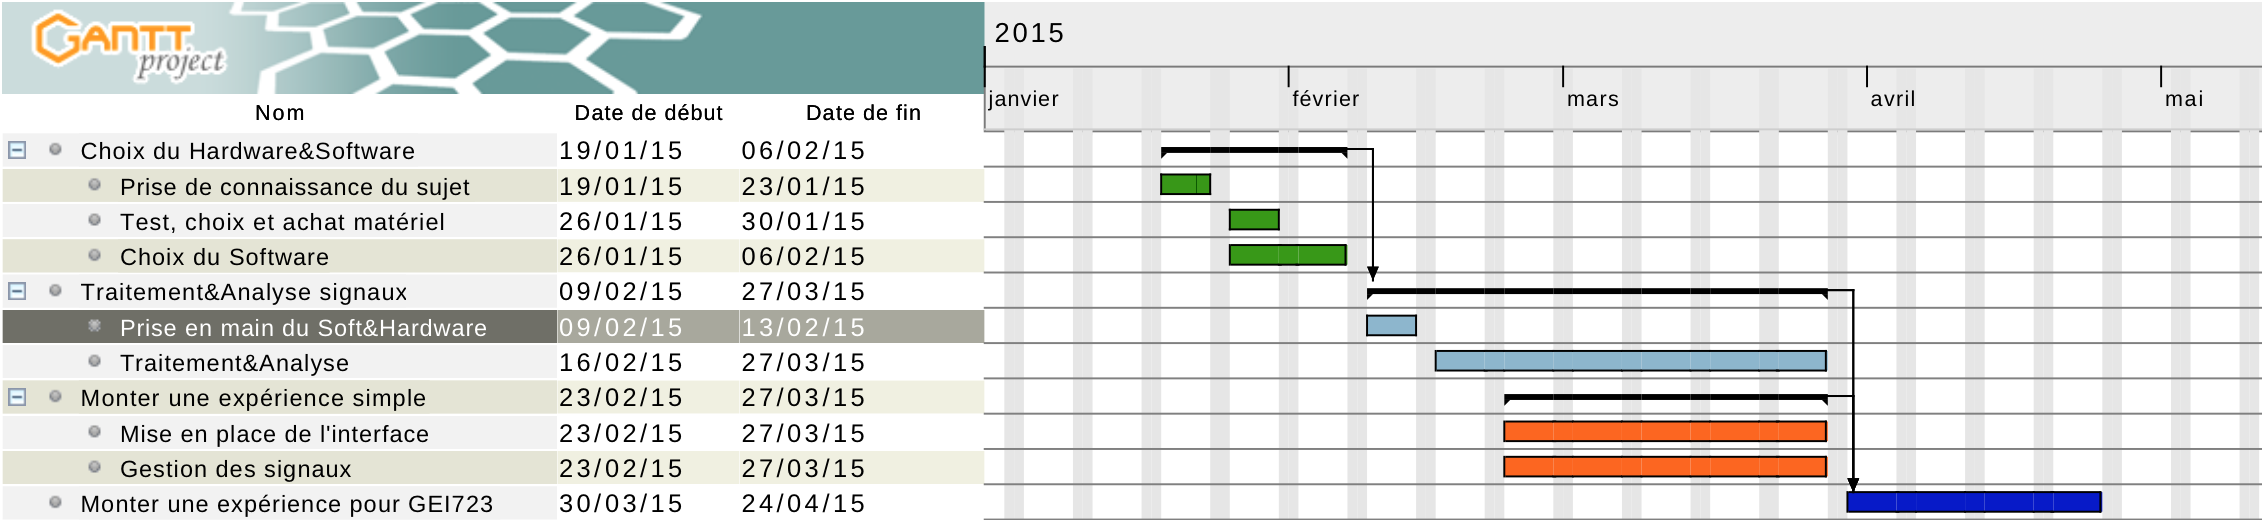
\includegraphics[width=15cm,height=6cm]{images/gant.png}
	\caption{Planning de Gantt prévisionnel}
\end{figure}
